\chapter{Setup}

% dark box
% power supplies
% multimeter
% osci
% gandalf + clock
% led + diffusor
% emusic
% sipm
In this chapter, the setup with which the different tests with the \ac{emusic} boards were performed is described.
First the \acp{sipm} and the \ac{sipm} boards is shown, then the dark box, in which the \ac{sipm} boards were placed for the tests.
Lastly the setup part with the \acp{gandalf} is described.

\section{SiPM}
An important part of the setup are of course the \acp{sipm} which generate the charge signal which than gets amplified by the \ac{emusic} chips.
The \acp{sipm} mainly used in this work are the \textit{S14160-3050HS} by the manufacturer Hamamatsu.
During the \ac{desy} testbeam also the SensL \textit{J-Series 30035} manufactured by Onsemi were used besides the \textit{S14160-3050HS}.
A few important parameters of both \ac{sipm} models are listed in \autoref{tab:sipm_specs}.
The \ac{sipm} boards which were used in this work have forty \acp{sipm} soldered onto them.
These boards exist with both \ac{sipm} models.
A picture of the front and back side of a Hamamatsu \ac{sipm} board is shown in \autoref{fig:sipm_pcb}.
A breakout board can be plugged in on the back of the \ac{pcb}.
For this thesis the \ac{emusic} board, which is described in the previous chapter, was plugged onto the \ac{sipm} board.
\begin{table}
	\centering
	\caption[SiPM parameters]{Relevant parameters of the both used \ac{sipm} models by Hamamatsu and Onsemi. \cite{HamamatsuSiPM,SensLSiPM}}
	\label{tab:sipm_specs}
	\renewcommand{\arraystretch}{1.3}
	\begin{tabularx}{\textwidth}{Xp{0.19\textwidth}p{0.15\textwidth}}
	    \toprule
	    parameter								& S14160-3050HS		& SensL			\\\midrule
	    photosensitive are / $\si{\milli\meter\squared}$			& 3.0$\times$3.0	& 3.07$\times$3.07	\\
	    pixel pitch / $\si{\micro\meter}$					& 50			& 35			\\
	    number of pixels							& 3000			& \num{5676}		\\
	    spectral response range / $\si{\nano\meter}$			& \numrange{270}{900}	& \numrange{200}{900}	\\
	    peak sensitivity wavenlength / $\si{\nano\meter}$			& 450			& 420			\\
	    breakdown voltage / $\si{\volt}$					& 38			& \numrange{24.2}{24.7}	\\
	    recommended operating voltage / $\si{\volt}$			& 40.7			& \numrange{25.2}{30.7}	\\
	    variation of rec. op. voltage (typ. / max) / $\si{\volt}$		& 0.1 / 0.2		&			\\
	    gain								& \num{2.5e6}		&			\\
	    \bottomrule
	\end{tabularx}
	\renewcommand{\arraystretch}{1}
\end{table} 
\begin{figure}
	\centering
	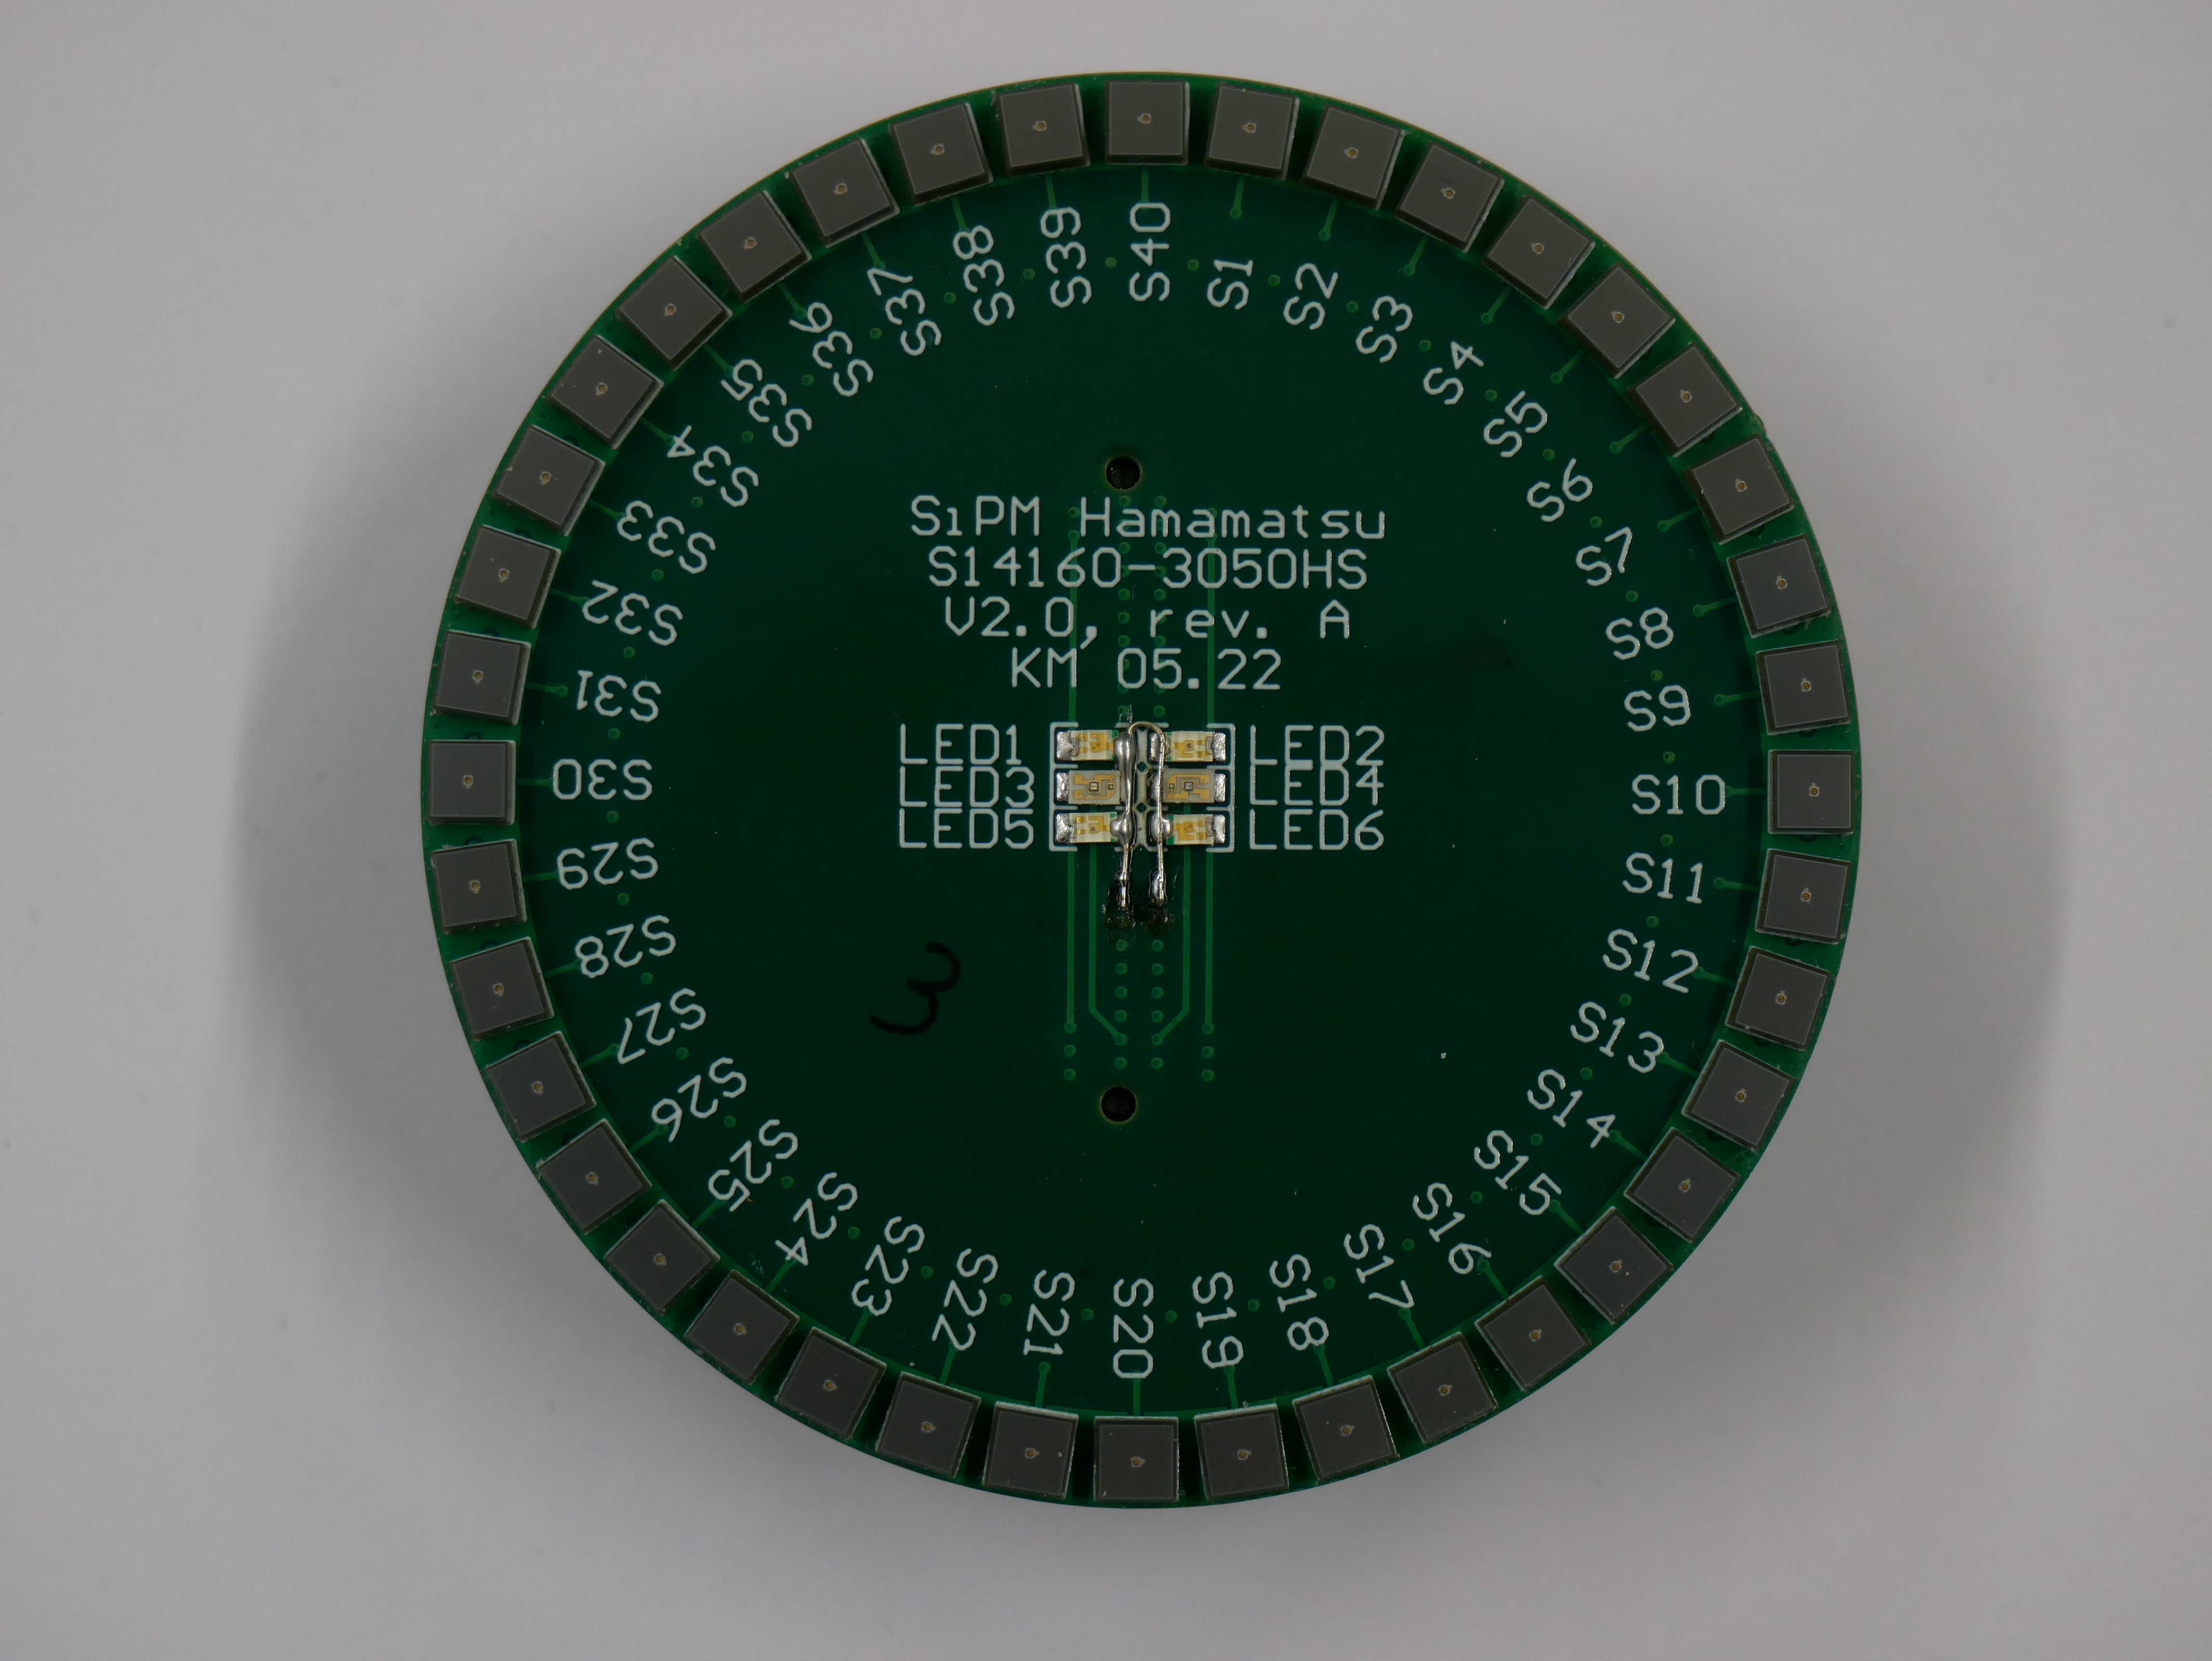
\includegraphics[width=.5\textwidth]{pictures/sipm_ham_pcb}
	\caption[\ac{pcb} with Hamamatsu \acp{sipm}]{One of the \acp{pcb} with Hamamatsu \acp{sipm} used for this work.}
	\label{fig:sipm_pcb}
\end{figure}

\section{Dark Box Setup}
To ensure a controlled evironment with controlled light exposure of the \acp{sipm} for the measurements, the \acp{sipm} were placed inside a dark box.
The inside of the box is covered in black aluminum foil made by Thorlabs with a reflectivity in the visible wavelength spectrum below \SI{5}{\percent} \cite{BKF12}.
An optical rail for fixing the \ac{sipm} board, a diffusor and the end of an optical fiber was placed in the box.
Via the optical fiber the light of a \SI{460}{\nano\meter} LED can be guided into the box.
The LED is inside of another light tight box.
It was build as part of the bachelor thesis of Alexander Bismark and is described there in more detail \cite{Bismark}.
Power can be supplied to the LED via a BNC connector on the light tight box.
In this thesis the Tektronix AFG was used to create voltage pulses with a width of \SI{4}{\nano\second} with \SI{2.5}{\nano\second} rising and falling edges.
To eluminate all \acp{sipm} equaly a \textit{ED1-C50-MD} diffuser by Thorlabs was used.
A light beam hitting the diffusor perpendicular to its surface gets diffused in a circular shape with a \SI{50}{\degree} opening angle.
%The relative light intensity of the diffused light of a collimated \SI{488}{\nano\meter} laser beam measured by Thorlabs is shown in \autoref{fig:diffuser_dist} \cite{}.

Multiple BNC, SMA, and SMC feedthroughs were installed in the dark box to supply the \acp{sipm} and \ac{emusic} board with power and to transfer the output signals of the \ac{emusic} out of the box to a digitizer or oscilloscope.
Also a hole drilled to insert the optical fiber from the LED setup into the box and afterwards covered, to block light from entering through the hole.
A power supply was used for the high voltage supply of the \acp{sipm}.
If not otherwise specified, all measurements shown in this thesis were done with a high voltage of \SI{43}{\volt}.
To control the voltage the HP multimeter was used instead of the less precise voltage display of the power supply.
The \ac{emusic} board was powered by a \SI{8}{\volt} power supply.
For the digitization either a \ac{gandalf} or the Tektronix oscilloscope was used.

\autoref{fig:setup_sketch} shows a schmatic sketch of the setup inside and on the outside of the box.
A picture of the setup inside the box is shown in \autoref{fig:setup_box_pic}.
It includes the LED fiber, the diffuser, the \ac{sipm} and \ac{emusic} board with power and signal cables attached.
In the following the setup part with the \ac{gandalf} is described.

\begin{figure}
	\centering
	\begin{circuitikz}
		\filldraw[fill=black!10!white, draw=black] (0,0) rectangle (5,8);
		\draw (1.6,5) rectangle (3.4,5.5) node[pos=.5] {SiPMs};
		\draw (1.6,5.7) rectangle (3.4,6.2) node[pos=.5] {eMUSIC};
		\draw (2.3,5.5) rectangle (2.7,5.7);
		\draw (2.2,3.1) rectangle (2.8,3.2) node[minimum width=.8cm, pos=.5,label={east:diffuser}] {};
		\shade[bottom color = blue, top color = blue!40!white] (2.55,3.2) -- (3.4,5) -- (1.6,5) -- (2.45,3.2) -- cycle ;
		\fill[fill=blue] (2.45,2.9) rectangle (2.55,3.1);
		\draw (2.4,2.4) rectangle (2.6,2.9) node[minimum width=.8cm, pos=.5,label={east:fiber end}] {};
		\draw (-6.,5.5) rectangle (-4.5,8) node[pos=.5, rotate=90] {GANDALF};
		\draw (-8.5,5.5) rectangle (-6.5,8) node[pos=.5, rotate=90] {computer};
		\draw[-latex] (2.5,6.2) -- (2.5,10.5) -- node[above] {signal x8} (-5.,10.5) -- (-5.,8);
		\draw[latex-] (3.,6.2) -- (3.,11.5) -- node[above] {eMUSIC configuration} (-5.3,11.5) -- (-8,11.5) -- (-8,8);
		\draw[-latex] (-5.5,8) -- (-5.5,10.5) -- node[above] {digitized} node[below] {data} (-7,10.5) -- (-7,8);
		\draw (-4,5.5) rectangle (-2.5,8) node[pos=.5, rotate=90] {HV supply};
		\draw (2,6.2) -- (2,9.5) -- (-3.25,9.5) -- (-3.25,8);
		\draw (-2,5.5) rectangle (-1,8) node[pos=.5, rotate=90] {LED box};
		\draw (2.5,2.4) -- (2.5,1.7) -- (.8,1.7) -- (.8,8.5) -- node[above] {optical fiber} (-1.5,8.5) -- (-1.5,8);
		\draw (-8.5,3) rectangle (-4.5,4.5) node[pos=.5, text width=3.5cm, align=center] {Tektronix AFG 3252};
		\draw (-1.5,5.5) -- (-1.5,3.75) -- (-4.5,3.75);
		\draw (-4.3,3.9) -- (-4.1,3.9) -- (-4.1,4.3) -- (-3.9,4.3) -- (-3.9,3.9) -- (-3.5,3.9);
	\end{circuitikz}
	\caption[Schematic view of the measurement setup.]{Schematic view of the measurement setup. The \ac{emusic} board and \ac{sipm} board are in a dark box to prevent unwanted light exposure. The high voltage for the \acp{sipm} is supplied by a power supply outide the box. An \SI{8}{\volt} power supply provides the power for the \ac{emusic} board. A computer is used to configer the \ac{emusic} chip. The output signals of the \ac{emusic} board are digitized by a\ac{gandalf} and then send to the computer, where they are written to disk. With voltage pulses from an arbitrary function generator a LED is powered. The emitted light is guided into the dark box through an optical fiber. In the box the fiber is mounted in front of the \acp{sipm} with a diffuser between the fiber end and the \acp{sipm}.}
	\label{fig:setup_sketch}
\end{figure}
\begin{figure}
	\centering
	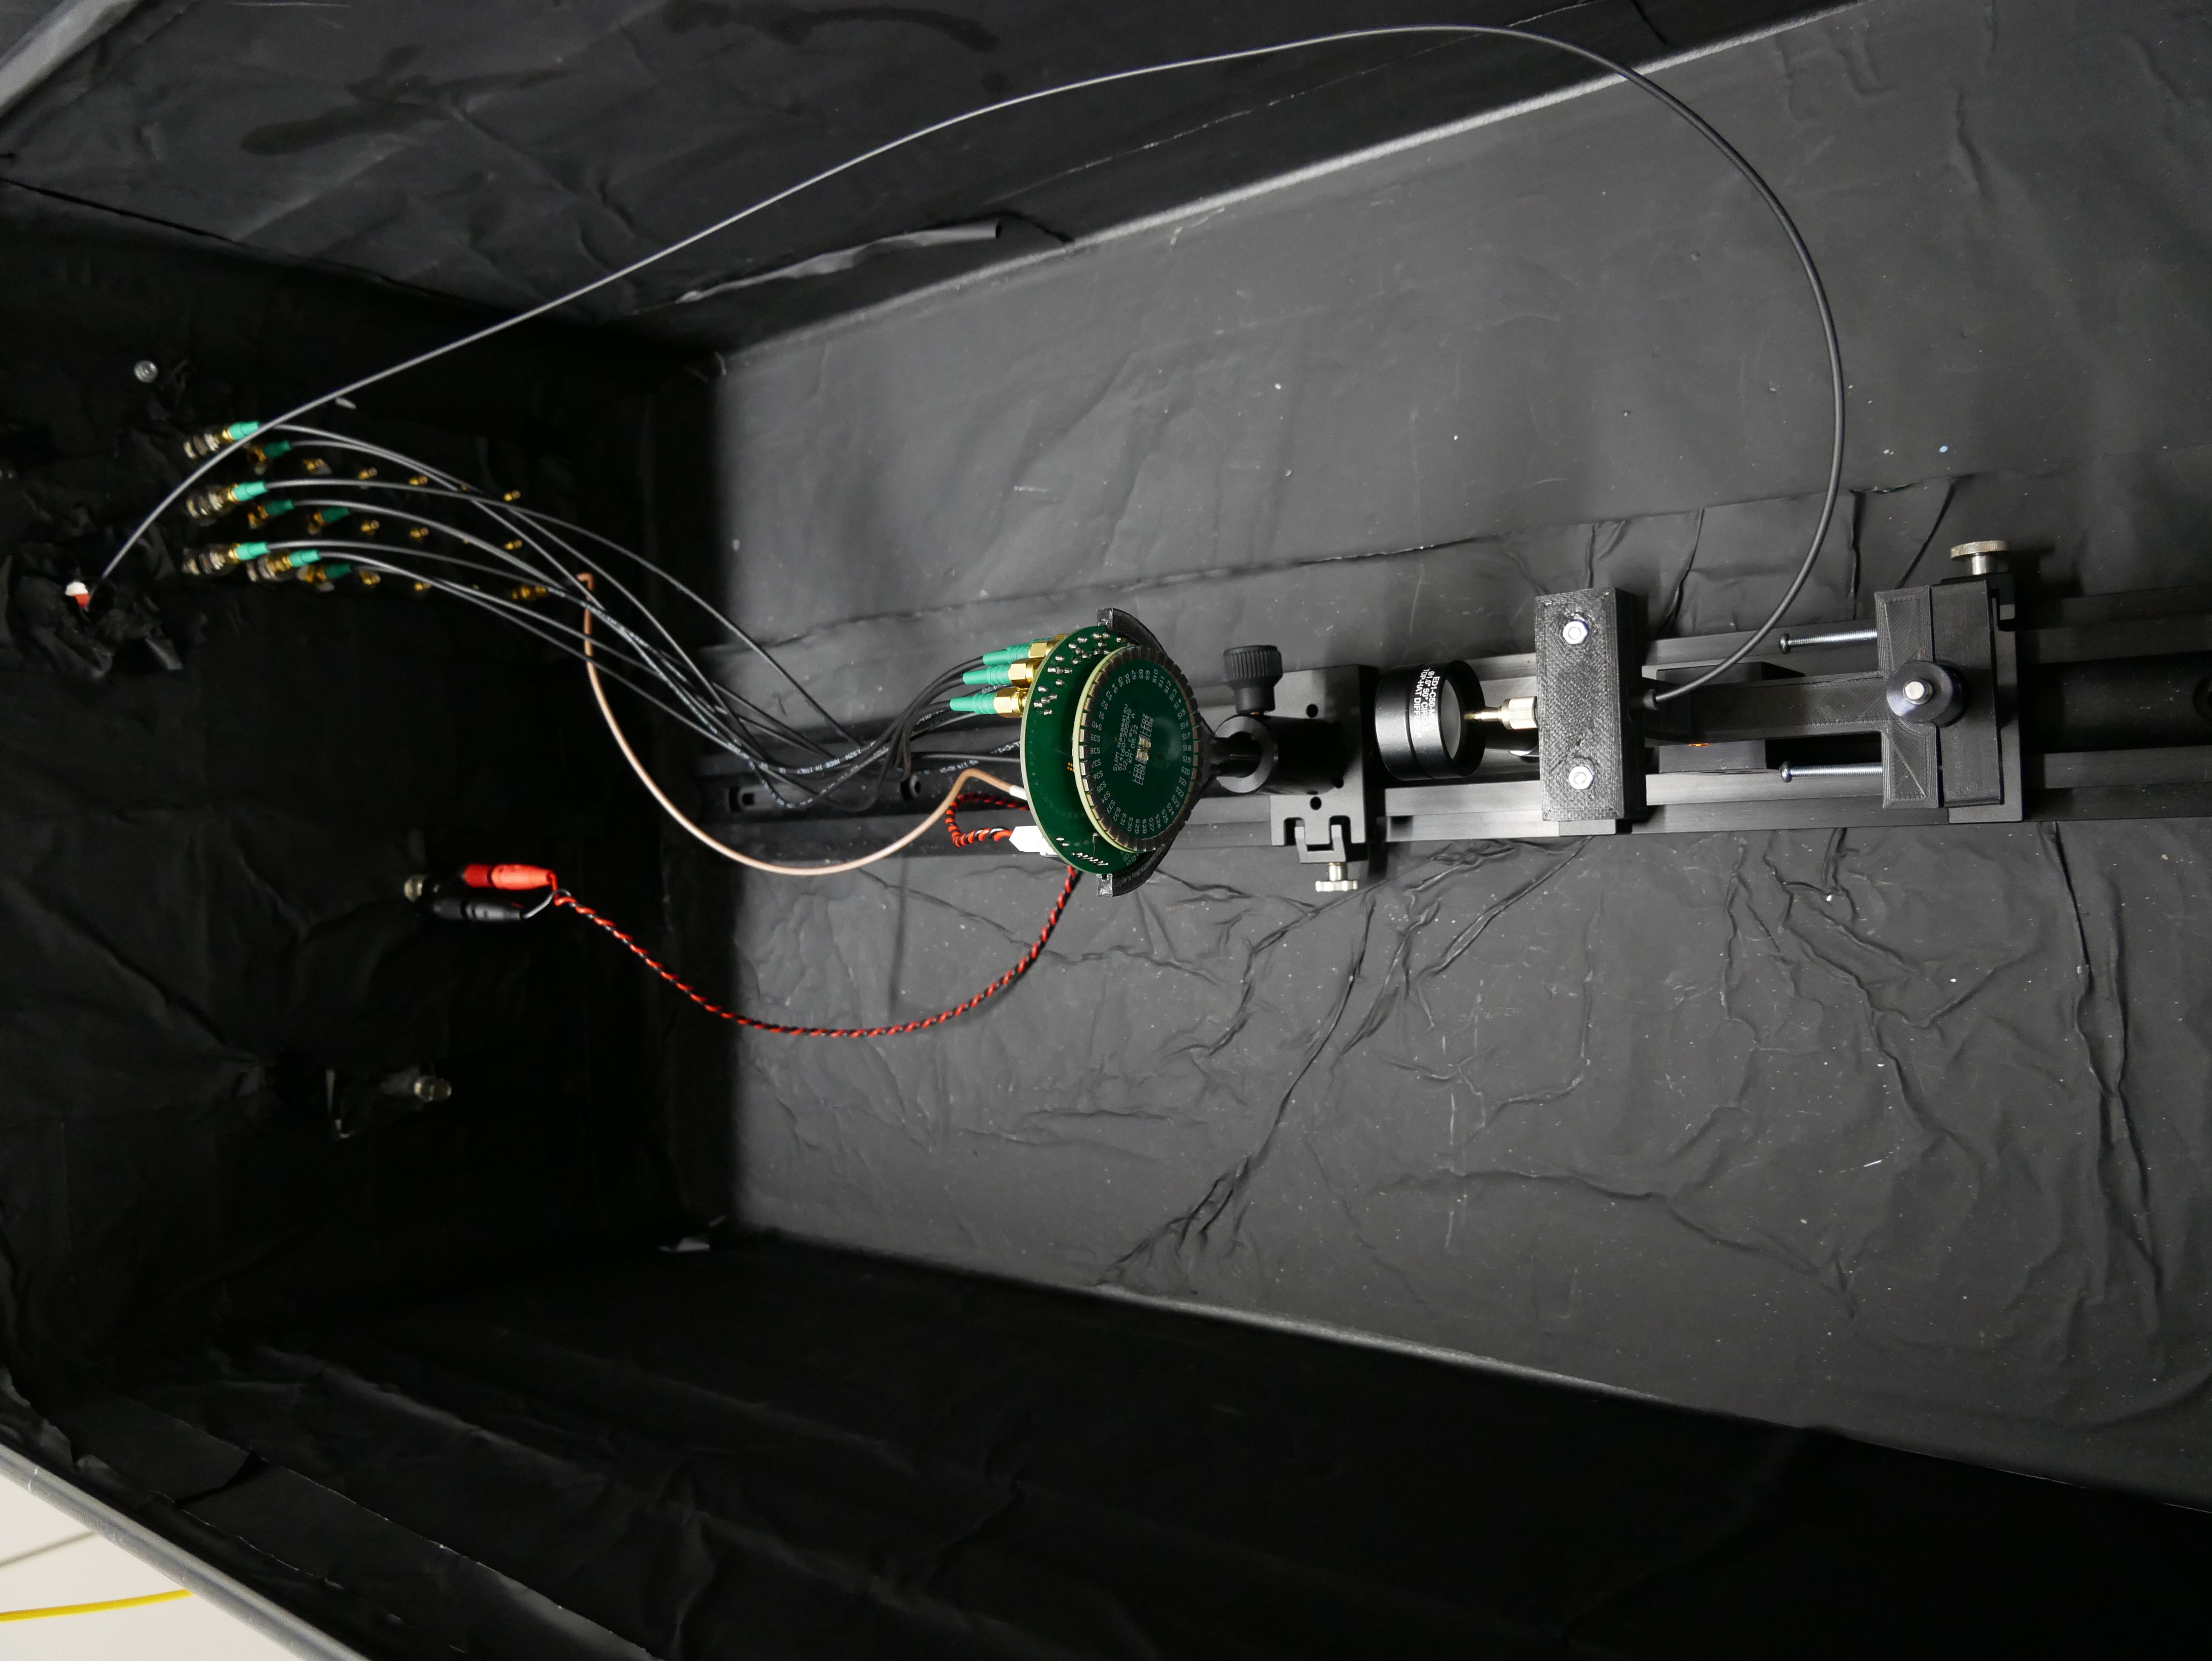
\includegraphics[width=0.5\textwidth]{pictures/setup_box_pic}
	\caption[Picture of the inside of the dark box.]{The inside of the dark box which was used for the test measurements. On the left is the end of the fiber from the LED setup mounted on the optical rail. Behind the fiber end is a diffuser by Thorlabs which diffuses the light in a circular distribution with an opening angle of \SI{50}{\degree}. After the diffuser is the \ac{pcb} with the \acp{sipm} placed. On its back is the \ac{emusic} board plugged in. The high voltage for the \acp{sipm} is supplied via the brownish cable, the power for the \ac{emusic} chip is supplied with the red and black cable and the signal outputs of the \ac{emusic} boards are connected with the feedthrough on the box via the black SMA cables.}
	\label{fig:setup_box_pic}
\end{figure}

\section{Gandalf}

For the operation of the One Cell Prototype sixteen channels need to be digitized, eight of each of the two \acp{wom}.
Therefore two \acp{gandalf} are required.
In order to save place and simplify the setup, the \acp{gandalf} are not operated in a VME crate but are each in a \ac{gandalf} portable.
It is a mobile case made exactly for such puroses where a whole crate is unconvinient to use.
A picture of a \ac{gandalf} portable is shown in \autoref{fig:gandalf_portable}.
Due to the usage of two \acp{gandalf} an external clock is required to ensure a syncronized sampling frequency and clock for time stamps.
As an external clock a copper GIMLI was chosen and used with a GIMLI testboard, shown in \autoref{fig:gimli_testboard}.
It has two slots for GMILIs with a clock output for each slot and a power connector to supply it with \SI{5}{\volt}.
For the purpose of an external clock, only one of these slots and the corresponding clock output is used.
Via LEMO cables, the clock signal form the boards clock output pins is connected to the clock inputs of the \acp{gandalf}.
\begin{figure}
	\centering
	\begin{subfigure}[b]{.4\textwidth}
		\centering
		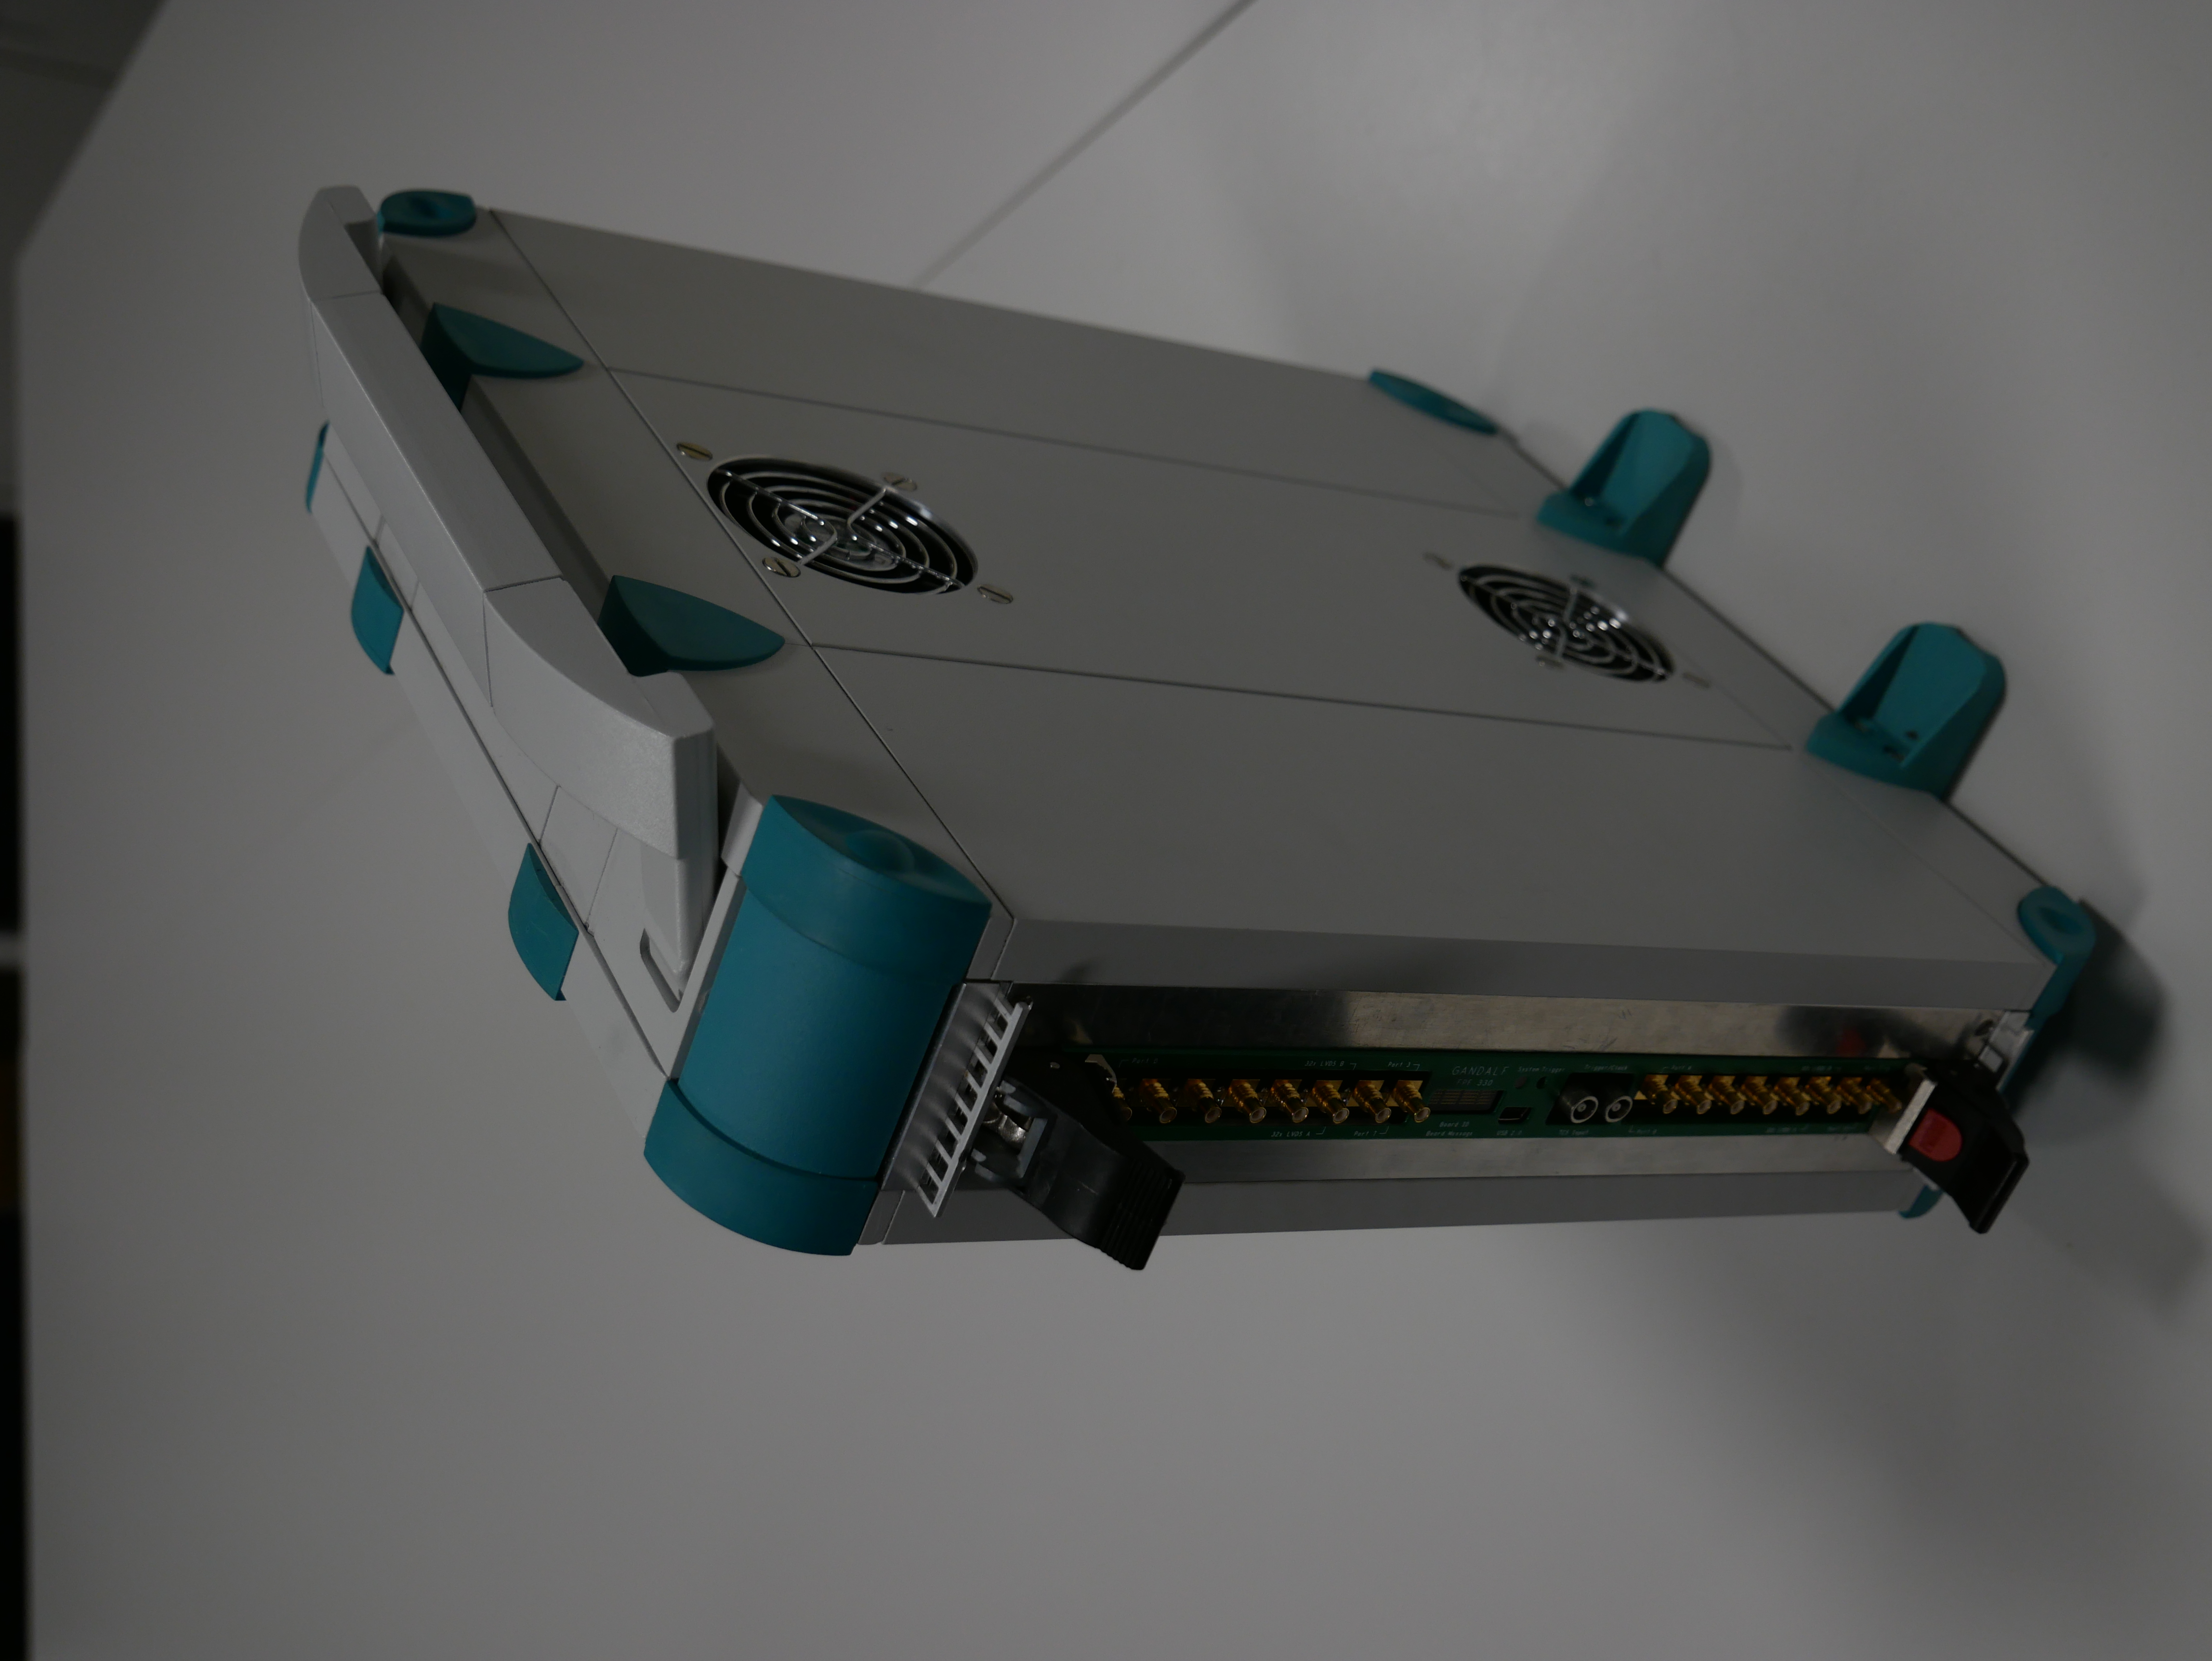
\includegraphics[width=1.\textwidth, angle=-90]{pictures/gandalf_portable} 
		\caption[A \ac{gandalf} portable equiped with a \ac{gandalf}.]{}
		\label{}
	\end{subfigure}
	\begin{subfigure}[b]{.55\textwidth}
		\centering
		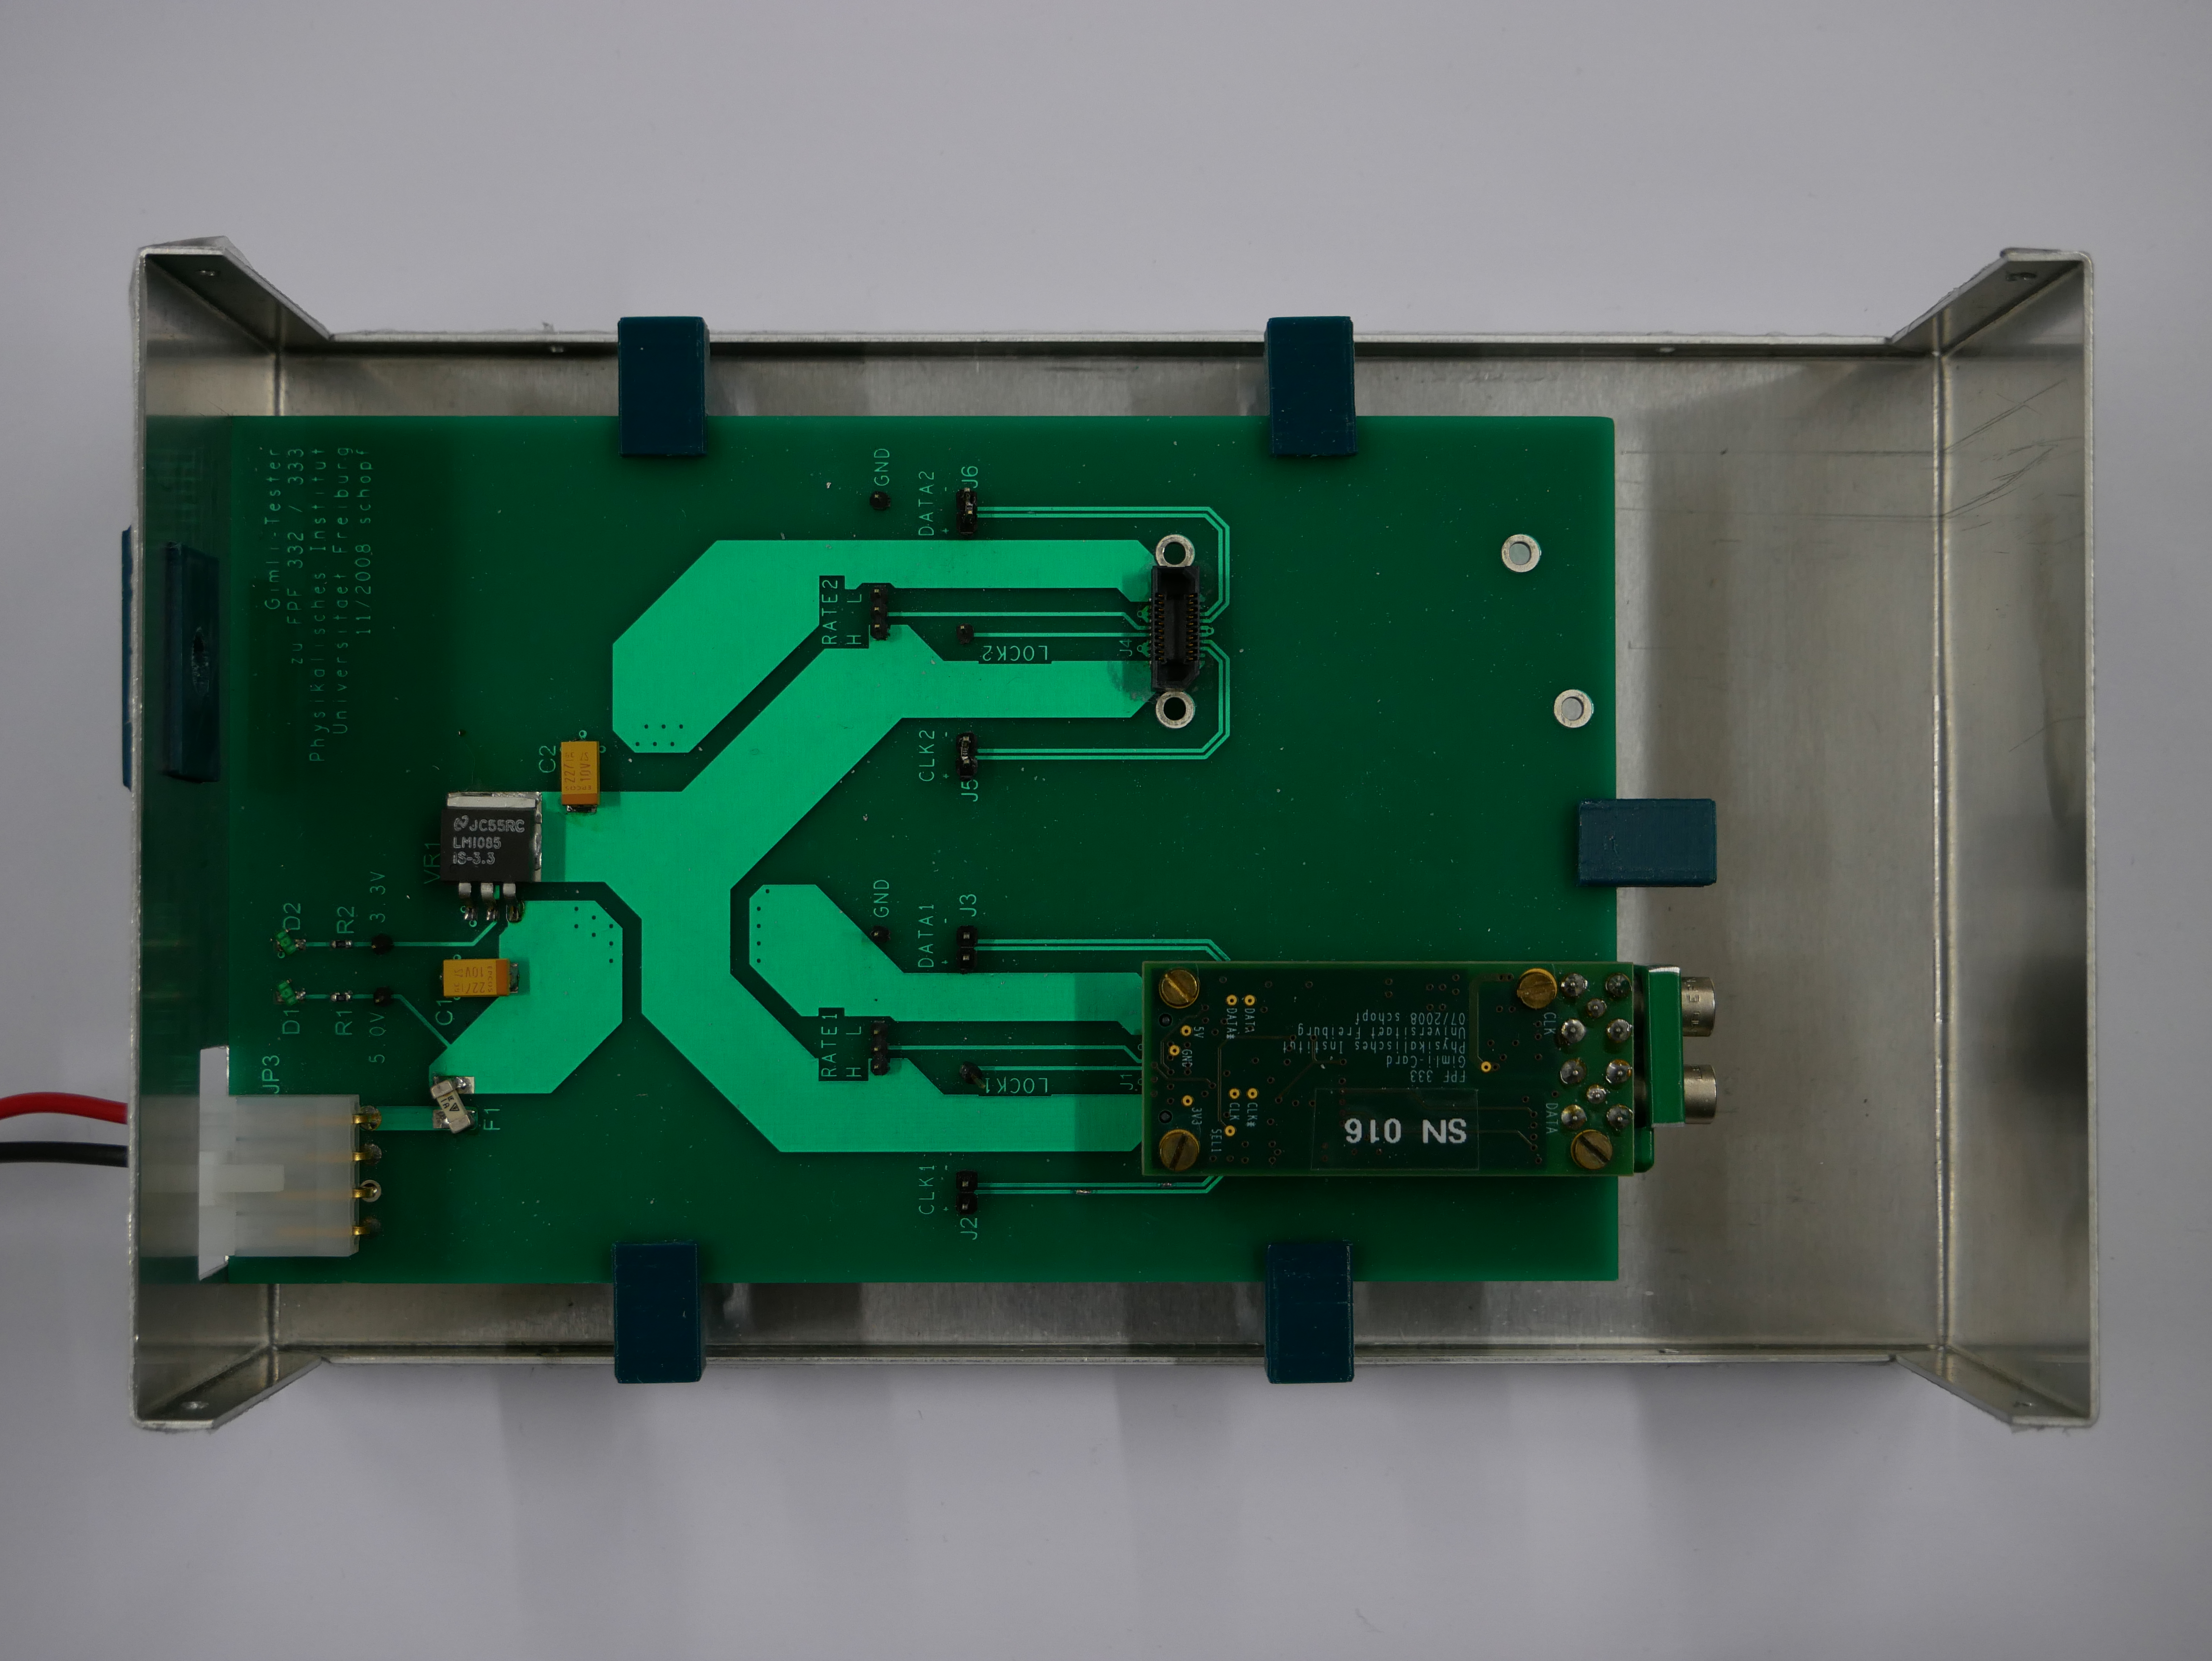
\includegraphics[width=1.\textwidth]{pictures/gimli_testboard}
		\caption[]{}
		\label{}
	\end{subfigure}
	\caption[]{A \ac{gandalf} portable equiped with a \ac{gandalf}. The GIMLI test board with a copper GIMLI}
	\label{}
\end{figure}
